\section{Yêu cầu đề tài}

\subsection{Mục tiêu thiết kế}
Thiết kế bộ điều khiển I2C Master tuân thủ chuẩn I2C dựa trên kiến trúc RD1139 của Lattice Semiconductor.

Hỗ trợ tốc độ 100 kHz (Standard Mode) và 400 kHz (Fast Mode).

Hỗ trợ các chế độ:
\begin{itemize}[leftmargin=1.2cm]
    \item Ghi dữ liệu (Write)
    \item Đọc dữ liệu (Read)
    \item Địa chỉ slave 7-bit
    \item Tạo và xử lý đầy đủ START, STOP, ACK/NACK, repeated START.
\end{itemize}

Đảm bảo hoạt động ổn định khi tích hợp vào SoC hoặc FPGA.

\subsection{Ràng buộc thiết kế}
Hoạt động theo chuẩn I2C:
\begin{itemize}[leftmargin=1.2cm]
    \item Tốc độ: 100 kHz (Standard), 400 kHz (Fast Mode).
    \item SDA phải thay đổi khi SCL = LOW.
    \item START: SDA đi từ HIGH $\rightarrow$ LOW khi SCL = HIGH.
    \item STOP: SDA đi từ LOW $\rightarrow$ HIGH khi SCL = HIGH.
    \item Tín hiệu SDA và SCL là open-drain (Inout).
    \item Hoạt động ổn định ở xung clock hệ thống 32 MHz.
    \item Được mô tả bằng Verilog/SystemVerilog HDL với testbench có sẵn.
\end{itemize}

\section{Mô tả thiết kế}

\subsection{Kiến trúc tổng thể}
Thiết kế bao gồm các module chính sau (được mô tả trong sơ đồ khối Figure 2.1 và 2.2):
\begin{itemize}[leftmargin=1.2cm]
    \item Processor Interface
    \item I2C Master Control FSM
    \item I2C Bus Control FSM
    \item Clock Generator \& Synchronizer
    \item Tx Data FSM \& Rx Data FSM
    \item Start/Stop detect \& generate logic
    \item Acknowledge logic
\end{itemize}

Hai FSM là thành phần quan trọng nhất:
\begin{itemize}[leftmargin=1.2cm]
    \item I2C Master Control FSM: điều khiển quá trình gửi/nhận từng byte.
    \item I2C Bus Control FSM: xử lý START, STOP, ACK và đồng bộ clock.
\end{itemize}

\begin{figure}[H]
    \centering
    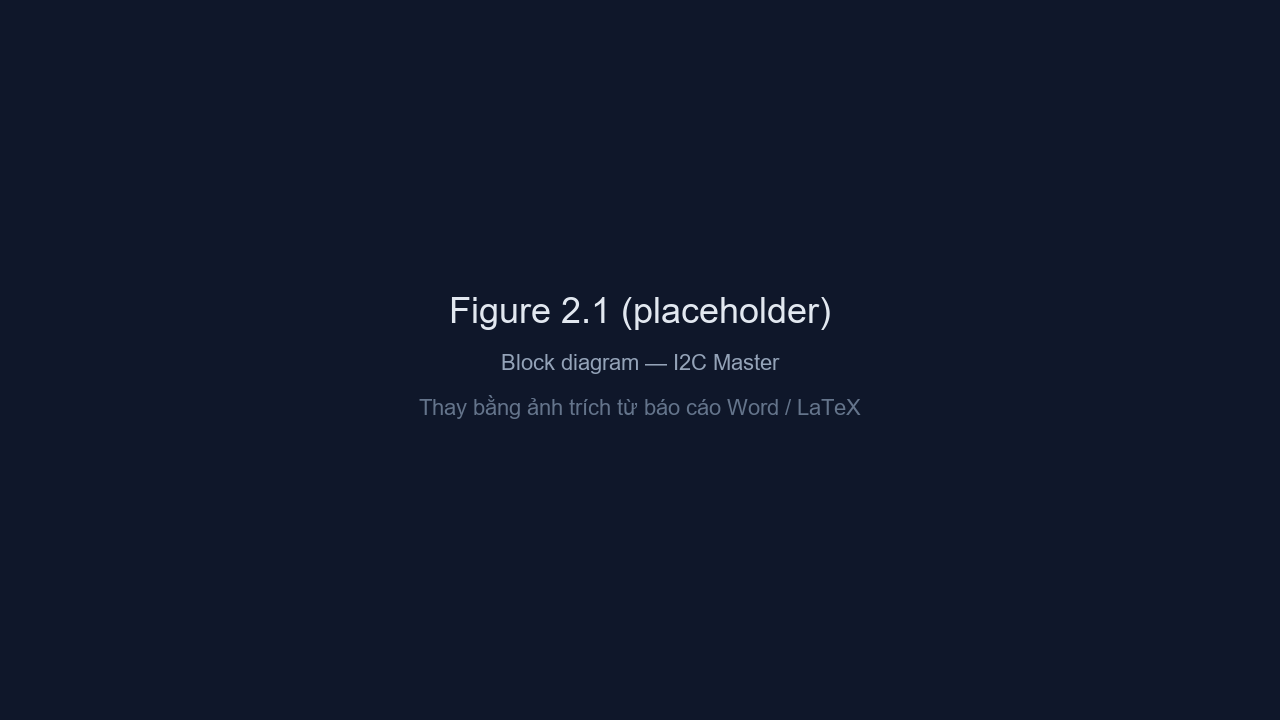
\includegraphics[width=0.92\textwidth,keepaspectratio]{figures/i2c_from_docx/fig01.png}
    \caption{I2C Master Controller Block Diagram}
    \label{fig:block}
\end{figure}

\subsection{Mô tả các thanh ghi}
\begin{table}[H]
    \centering
    \caption{Register Description}
    \label{tab:reg}
    \begin{tabularx}{\textwidth}{|l|X|}
        \hline
        \textbf{Thanh ghi} & \textbf{Chức năng} \\
        \hline
        \texttt{i\_slave\_addr\_reg} & Địa chỉ 7-bit của slave. \\
        \hline
        \texttt{i\_byte\_cnt\_reg} & Số byte cần truyền/nhận. \\
        \hline
        \texttt{i\_clk\_div\_lsb} + \texttt{i\_mode\_reg[2:0]} & Bộ chia clock tạo SCL. \\
        \hline
        \texttt{i\_config\_reg} & Gồm các bit START, INT\_CLR, TX\_IE, RX\_IE, ABORT, RESET. \\
        \hline
        \texttt{o\_cmd\_status\_reg} & TX\_DONE, RX\_DONE, TX\_ERR, RX\_ERR, ABORT\_ACK, I2C\_BUSY. \\
        \hline
    \end{tabularx}
\end{table}

\section{Nguyên lý hoạt động}

\subsection{Quá trình ghi (Master Transmit)}
Viết START = 1 trong \texttt{i\_config\_reg} để bắt đầu giao dịch.

\texttt{I2C\_BUSY} được set lên trước khi START bị auto-clear.

Trình tự:
\begin{itemize}[leftmargin=1.2cm]
    \item START.
    \item Gửi địa chỉ + bit R/W = 0.
    \item Slave trả lại ACK địa chỉ.
    \item Gửi từng byte dữ liệu.
    \item Slave trả lại ACK mỗi byte dữ liệu.
    \item STOP
\end{itemize}

\texttt{TX\_DONE} được set sau khi byte cuối được gửi.

\texttt{I2C\_BUSY} chỉ clear khi STOP hoàn tất.

\subsection{Quá trình đọc (Master Receive)}
Tương tự truyền, nhưng bit R/W = 1.

Byte dữ liệu từ slave được lấy vào \texttt{o\_receive\_data}, với \texttt{o\_received\_data\_valid} = 1.

Khi byte cuối đến, \texttt{RX\_DONE} được set.

\subsection{Repeated START}
Cho phép truy cập thanh ghi bên trong slave.

Trong lần START thứ hai, phải giữ nguyên địa chỉ slave.

Lặp lại trình tự START mà không cần tạo STOP giữa chừng.

\section{Sơ đồ RTL}

\begin{figure}[H]
    \centering
    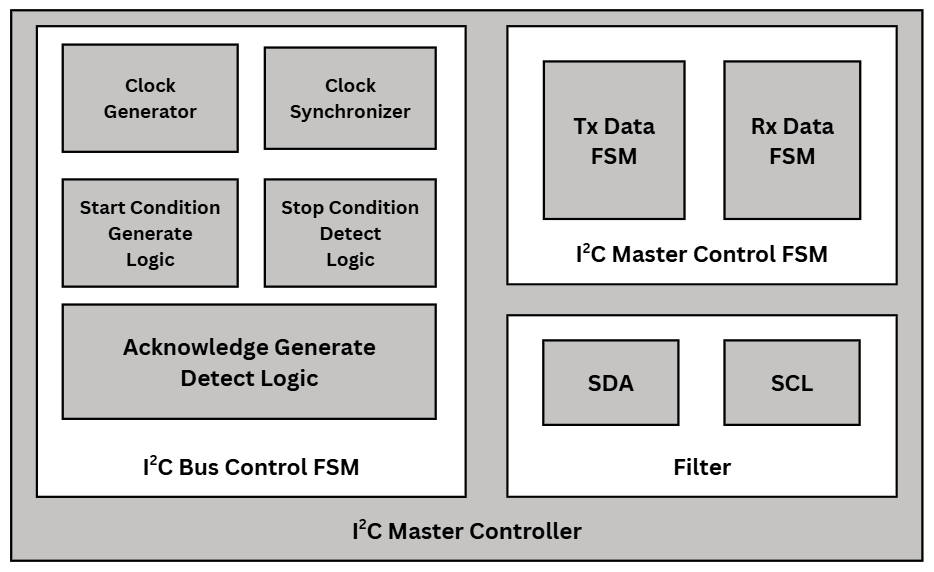
\includegraphics[width=0.92\textwidth,keepaspectratio]{figures/i2c_from_docx/fig02.png}
    \caption{RTL Functional Block Diagram}
    \label{fig:rtl}
\end{figure}

\subsection{Clock Generator/Synchronizer}
Dựa trên \texttt{i\_clk\_div\_lsb} và \texttt{i\_mode\_reg[2:0]} để tạo tần số SCL.

Đồng bộ hóa xung clock giữa master và slave theo cơ chế ``clock stretching''.

\subsection{I2C Bus Control FSM}
Sinh START/STOP theo điều kiện SDA thay đổi khi SCL HIGH.

Phát hiện START/STOP do slave tạo (multi-master).

Sinh/nhận ACK theo từng byte.

\begin{figure}[H]
    \centering
    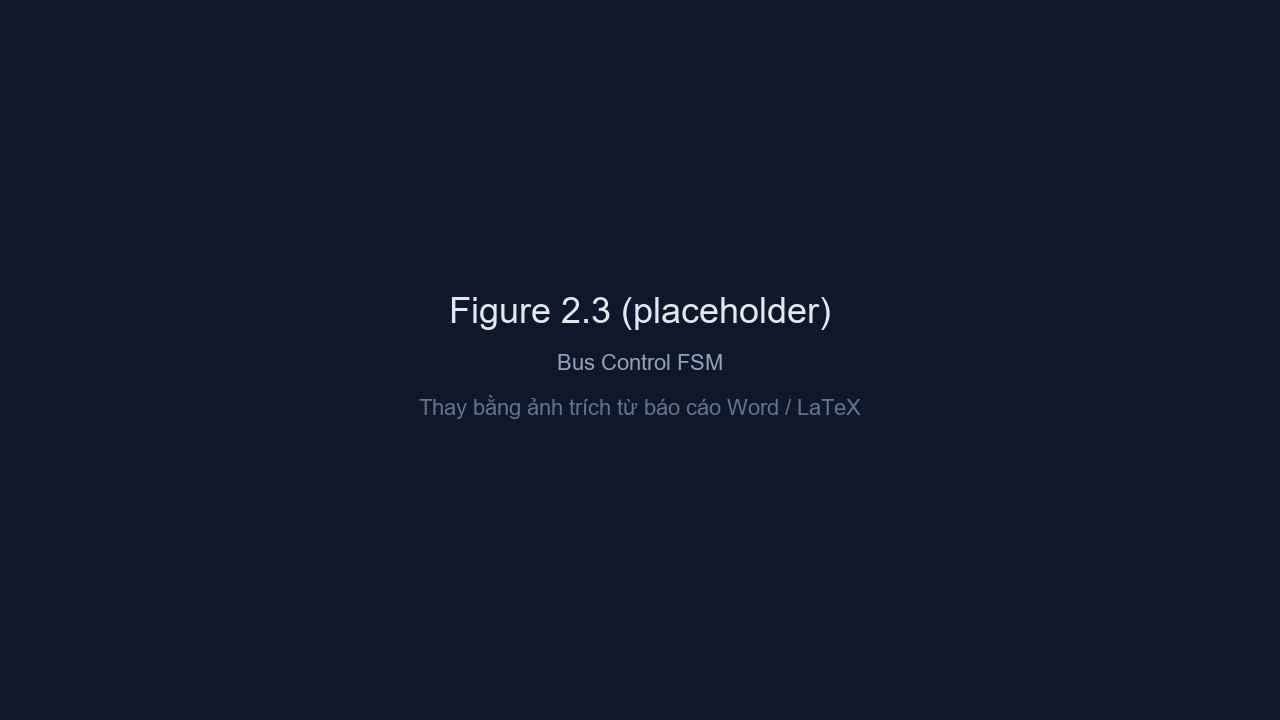
\includegraphics[width=0.88\textwidth,keepaspectratio]{figures/i2c_from_docx/fig03.png}
    \caption{I2C Bus Control FSM}
    \label{fig:bus_fsm}
\end{figure}

\subsection{I2C Master Control FSM}
FSM Chính điều khiển byte-level:
\begin{itemize}[leftmargin=1.2cm]
    \item IDLE
    \item START
    \item SEND\_ADDR
    \item ADDR\_ACK
    \item TX\_DATA/RX\_DATA
    \item DATA\_ACK
    \item STOP
    \item DONE
\end{itemize}

\begin{figure}[H]
    \centering
    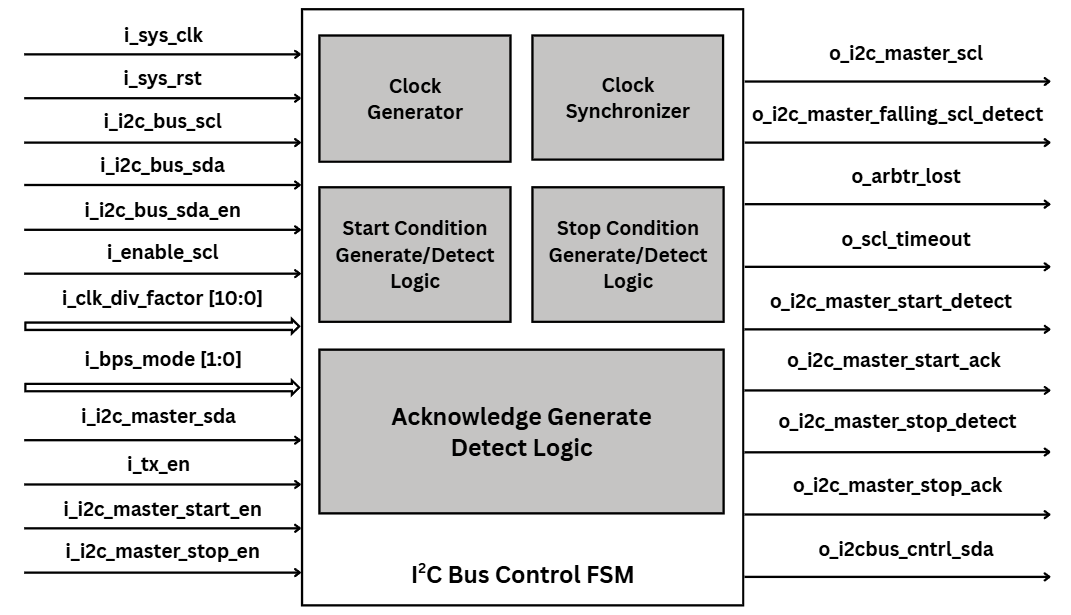
\includegraphics[width=0.88\textwidth,keepaspectratio]{figures/i2c_from_docx/fig04.png}
    \caption{I2C Master Control FSM}
    \label{fig:master_fsm}
\end{figure}

\subsection{Bộ đếm byte (Byte Counter)}
8-bit counter tăng sau mỗi byte được gửi/nhận.

So sánh với \texttt{i\_byte\_cnt\_reg} để xác định khi nào STOP phải được tạo.

\section{Mô phỏng thiết kế}

\subsection{Môi trường mô phỏng}
Testbench Verilog có sẵn trong RD1139.

Gồm mô phỏng đọc và ghi dữ liệu, cũng như repeated start.

\subsection{Kịch bản mô phỏng}

\subsubsection{Transmit Operation}
Quan sát các tín hiệu:
\begin{itemize}[leftmargin=1.2cm]
    \item START
    \item Địa chỉ + ACK
    \item Byte truyền
    \item STOP
\end{itemize}

Kết quả mong đợi:
\begin{itemize}[leftmargin=1.2cm]
    \item \texttt{o\_transmit\_data\_requested} được kích hoạt trước mỗi byte.
    \item \texttt{TX\_DONE} = 1 sau byte cuối.
\end{itemize}

\subsubsection{Receive Operation}
Quan sát:
\begin{itemize}[leftmargin=1.2cm]
    \item START
    \item READ
    \item Dữ liệu nhận \texttt{o\_receive\_data}
    \item STOP
\end{itemize}

\begin{itemize}[leftmargin=1.2cm]
    \item \texttt{o\_receive\_data\_valid} = 1 khi dữ liệu hợp lệ.
    \item \texttt{RX\_DONE} = 1 sau byte cuối.
\end{itemize}

\subsubsection{Repeated START}
Tạo START $\rightarrow$ Gửi địa chỉ $\rightarrow$ ACK.

Không tạo STOP.

Tạo START lần hai.

Slave trả dữ liệu.

\subsection{Waveform}

\begin{figure}[H]
    \centering
    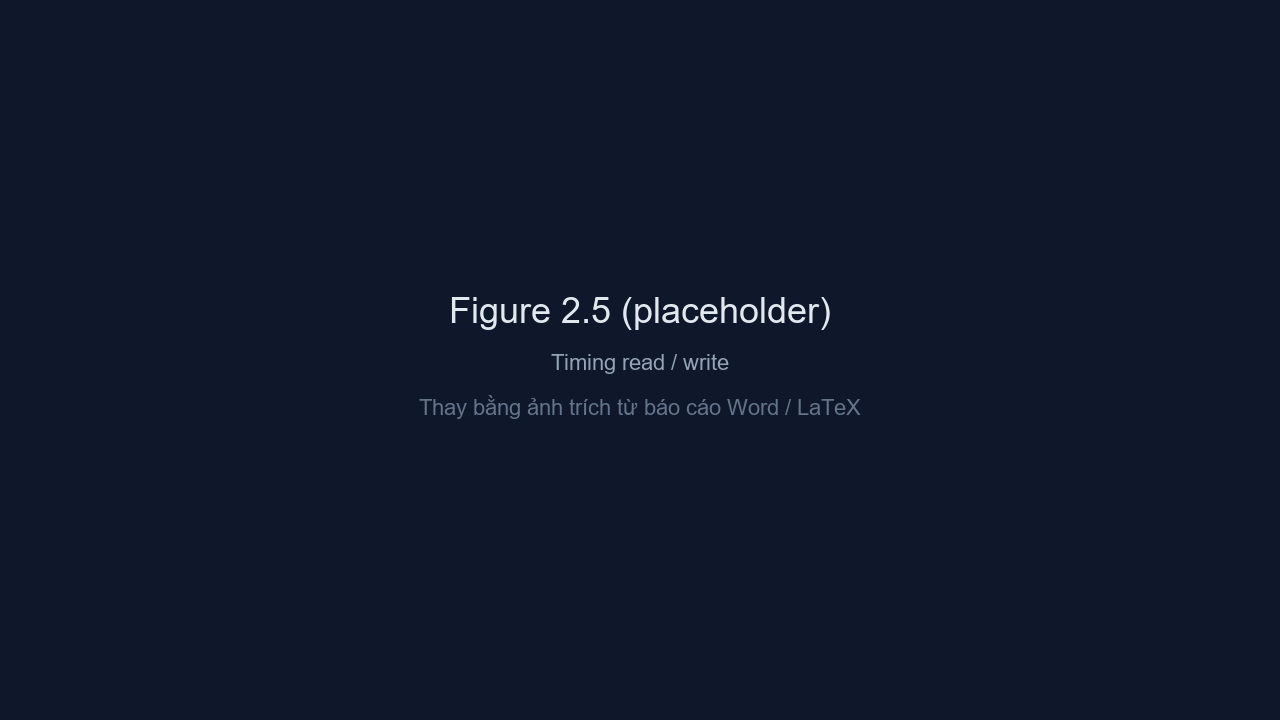
\includegraphics[width=0.95\textwidth,keepaspectratio]{figures/i2c_from_docx/fig05.png}
    \caption{Timing Diagram for Read and Write Data Transfer}
    \label{fig:w5}
\end{figure}

\begin{figure}[H]
    \centering
    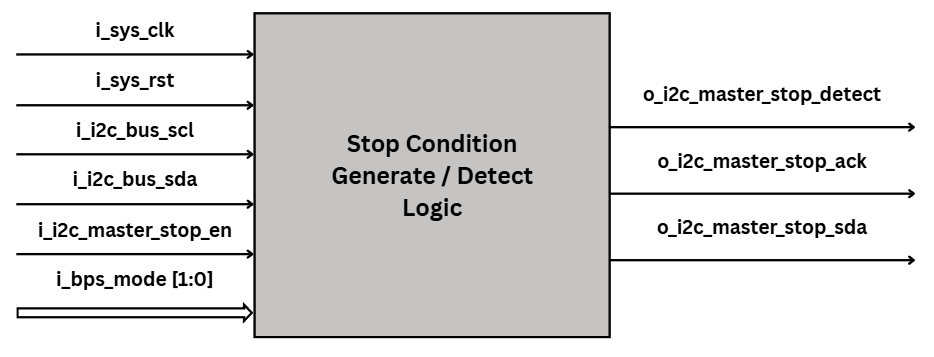
\includegraphics[width=0.95\textwidth,keepaspectratio]{figures/i2c_from_docx/fig06.png}
    \caption{Master Transmit Operation}
    \label{fig:w6}
\end{figure}

\begin{figure}[H]
    \centering
    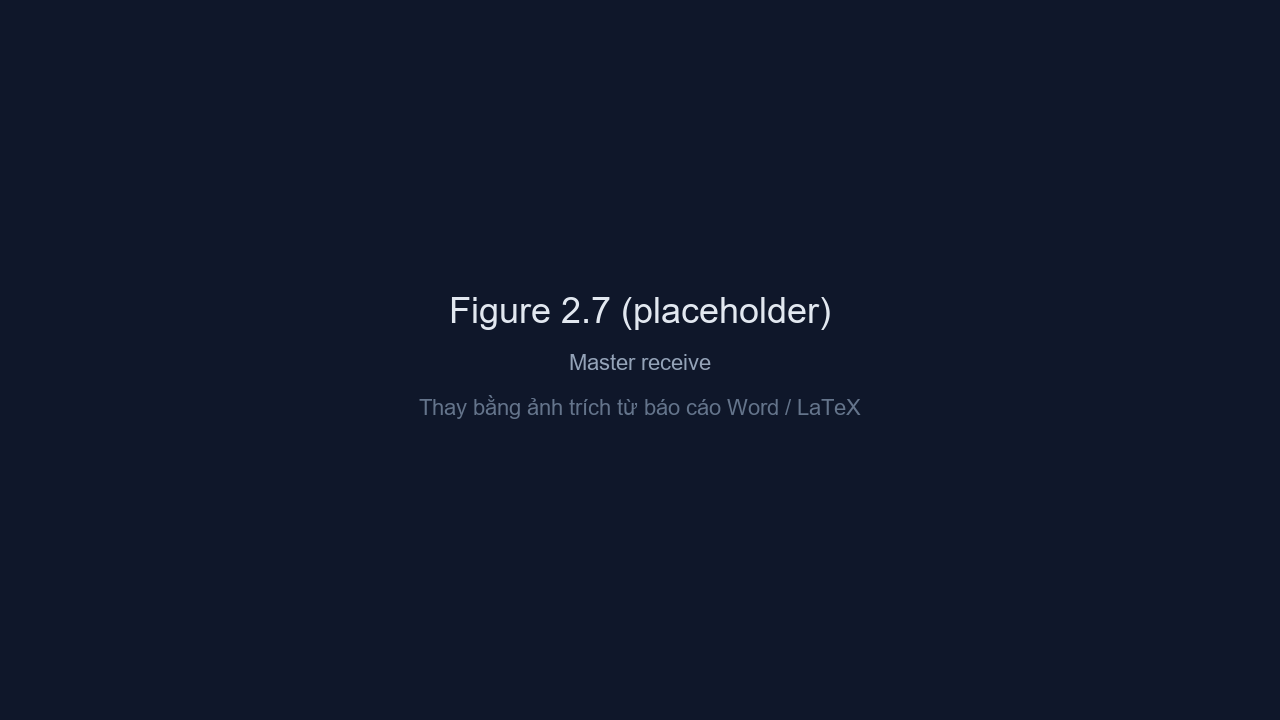
\includegraphics[width=0.95\textwidth,keepaspectratio]{figures/i2c_from_docx/fig07.png}
    \caption{Master Receive Operation}
    \label{fig:w7}
\end{figure}

\begin{figure}[H]
    \centering
    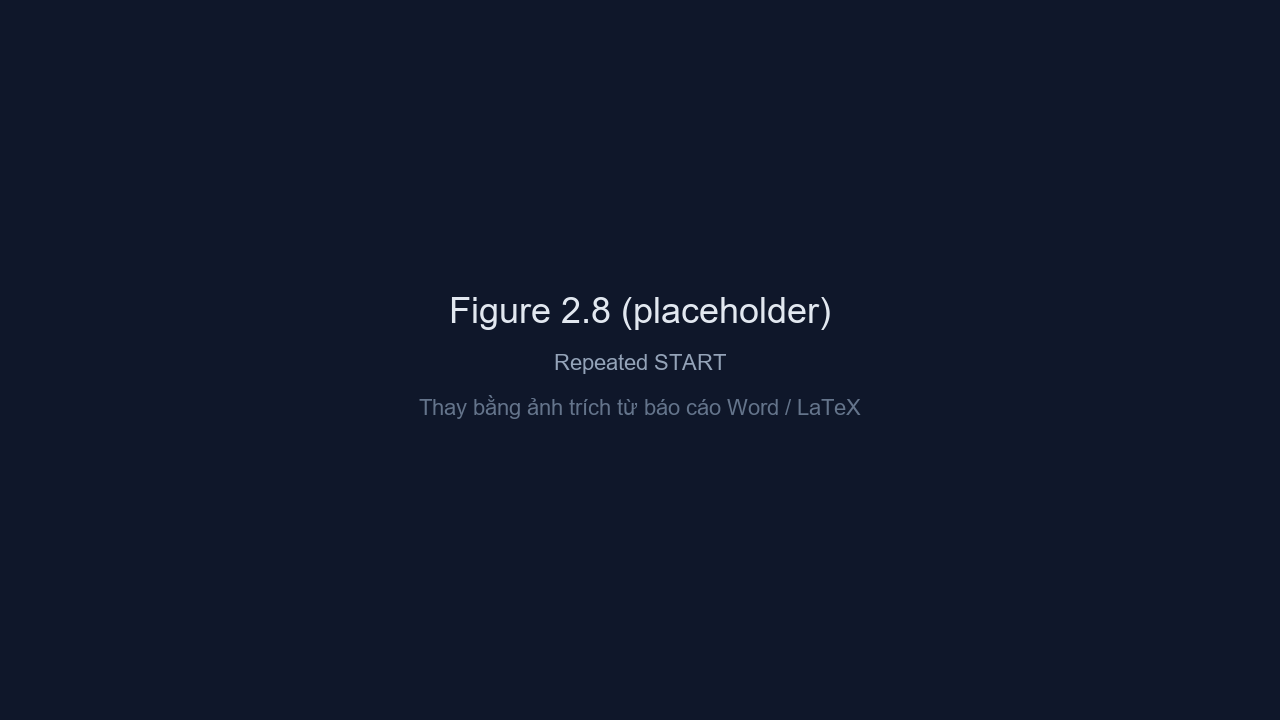
\includegraphics[width=0.95\textwidth,keepaspectratio]{figures/i2c_from_docx/fig08.png}
    \caption{Repeated Start Operation}
    \label{fig:w8}
\end{figure}
